\documentclass[compact]{ne630handout}
\HandoutTypography{9}{10.7}{5pt}

\handoutsolutionsfalse
% Uncomment to reveal numerical answers and instructor cues.
% \handoutsolutionstrue
\ifdefined\instructorsolutions\handoutsolutionstrue\fi

\hypersetup{pdftitle={NE 630 -- Lesson 27: One-Group Delayed-Neutron Kinetics},
  pdfauthor={Jeremy Roberts}}

\begin{document}
\Lesson{27}{One-Group Delayed-Neutron Kinetics}{FNRP 5.4; one-group results from 5.5.}
{Relate a physical precursor concentration to $(n,C)$, find a critical equilibrium,
and infer reactivity from neutron-density traces.}

\begin{handoutflow}
\Sec{1}{One physical precursor}

Use \textbf{bromine-87} as the only delayed-neutron precursor.
Treat all remaining fission neutrons as prompt; neglect precursor capture
and parent ingrowth. Here, \emph{one group} means one precursor group.
\[
 {}^{87}\mathrm{Br}\xrightarrow{\beta^-}{}^{87}\mathrm{Kr}^{*}
       \xrightarrow{n}{}^{86}\mathrm{Kr}.
\]
Use the following data:
\[
 \begin{array}{rlrl}
 \gamma&=0.01274\ {\rm nuclei/fission},&
 f_n&=0.0260,\\
 t_{1/2}&=55.65\ {\rm s},&
 \bar\nu&=2.43.
 \end{array}
\]
Here $f_n$ is the probability that a Br-87 decay produces a neutron.
For the \textbf{actual} Br-87 number density $N(t)$,
\[
 \frac{dN}{dt}=\gamma\Sigma_f\phi-\lambda N,
 \qquad \lambda=\frac{\ln 2}{t_{1/2}},
\]
and the delayed-neutron production rate is $f_n\lambda N$.
\SourceLine{Br-87 decay reference: P. Dimitriou et al.,
\href{https://doi.org/10.1016/j.nds.2021.04.006}
{\emph{Nuclear Data Sheets} 173, 144--238 (2021)},
Table XXIII, ENDF/B-VIII.0 column ($t_{1/2}=55.65$ s, $f_n=0.026$).}

\Sec{2}{The classic $(n,C)$ equations}

Define the delayed-neutron-equivalent concentration and delayed fraction:
\[
 \boxed{C=f_nN,\qquad N=\frac{C}{f_n}},\qquad
 \beta=\frac{f_n\gamma}{\bar\nu}=1.3631\times10^{-4}.
\]
$C$ counts the \emph{expected} future delayed neutrons per unit volume;
it is not the total number density of Br-87.
With $\phi=\bar v n$ and $\Lambda=(\bar\nu\Sigma_f\bar v)^{-1}$,
\begin{equation*}
 \boxed{\begin{aligned}
 \frac{dn}{dt}&=\frac{\rho(t)-\beta}{\Lambda}\,n+\lambda C+S(t),\\
 \frac{dC}{dt}&=\frac{\beta}{\Lambda}\,n-\lambda C .
 \end{aligned}}
\end{equation*}
$n,C,N$ have units cm$^{-3}$; $S$ has units cm$^{-3}$s$^{-1}$.
The reactivity is $\rho=(k-1)/k$.
Identify prompt production minus loss, delayed production, and precursor loss.

\Sec{3}{Critical steady state, with $S=0$}

Set both derivatives to zero:
\[
 C_0=\frac{\beta n_0}{\lambda\Lambda},\qquad
 0=\frac{\rho-\beta}{\Lambda}n_0+\lambda C_0
   =\frac{\rho}{\Lambda}n_0.
\]
Thus a nonzero source-free equilibrium requires \textbf{$\rho=0$}.
Its amplitude $n_0$ must be specified by the operating density or power.
The corresponding physical precursor concentration is
\[
 \boxed{N_0=\frac{C_0}{f_n}
       =\frac{\gamma\Sigma_f\phi_0}{\lambda}.}
\]
\textbf{Check.} For $n_0=10^8$ cm$^{-3}$ and
$\Lambda=5\times10^{-5}$ s, calculate
\[
 C_0=\RevealMath[1.08in]{2.189\times10^{10}}\ {\rm cm}^{-3},\qquad
 N_0=\RevealMath[1.08in]{8.418\times10^{11}}\ {\rm cm}^{-3}.
\]
Why can the precursor inventory greatly exceed the neutron inventory?

\columnbreak
\Sec{4}{A step produces two exponential modes}

Start at the critical equilibrium above. At $t=0$, impose a constant
$\rho$ while keeping $S=0$ and the material parameters fixed:
\[
 \frac{d}{dt}\begin{bmatrix}n\\ C\end{bmatrix}
 =
 \begin{bmatrix}
  (\rho-\beta)/\Lambda & \lambda\\
  \beta/\Lambda &-\lambda
 \end{bmatrix}
 \begin{bmatrix}n\\ C\end{bmatrix}.
\]
For a mode proportional to $e^{\omega t}$, the eigenvalues satisfy
\[
 \boxed{\Lambda\omega^2+
  (\beta-\rho+\lambda\Lambda)\omega-\lambda\rho=0.}
\]
For the sub-prompt-critical insertions used below, call the larger root
$\omega_s$ and the smaller root $\omega_f$. Then
\[
 n(t)=A_s e^{\omega_s t}+A_f e^{\omega_f t}.
\]
The initial conditions give
\[
 A_s+A_f=n_0,\qquad
 \omega_s A_s+\omega_f A_f=\frac{\rho}{\Lambda}n_0.
\]
The fast mode dies away first. Both $n$ and $C$ remain \textbf{continuous}
at $t=0$; their derivatives can change immediately.

\Sec{5}{Measure the late-time period}

After the fast mode has become negligible,
\[
 n(t)\simeq A_s e^{t/T},\qquad \boxed{T=\frac{1}{\omega_s}}.
\]
Choose two points on the straight, late part of a semilog trace:
\[
 \boxed{T=\frac{t_b-t_a}{\ln[n(t_b)/n(t_a)]}.}
\]
$T>0$ means growth; $T<0$ means decay. A population doubles in
$T\ln 2$ for $T>0$, or halves in $|T|\ln 2$ for $T<0$.
Substituting $\omega=1/T$ into the quadratic gives a direct
\textbf{one-group period--reactivity relation}:
\[
 \boxed{\rho=\frac{\Lambda}{T}+\frac{\beta}{1+\lambda T}.}
\]
This is the one-group version of the \emph{inhour} equation.

\Sec{6}{Estimate the prompt jump or drop}

For a step sufficiently below prompt criticality, $C$ changes little
during the fast adjustment. Set $dn/dt\simeq0$ while retaining $C\simeq C_0$:
\[
 0\simeq\frac{\rho-\beta}{\Lambda}n_1+\lambda C_0
 \quad\Longrightarrow\quad
 \boxed{J\equiv\frac{n_1}{n_0}\simeq\frac{\beta}{\beta-\rho}.}
\]
Consequently, $\rho/\beta\simeq1-1/J$. The apparent jump describes
a short, continuous adjustment; it is not $n(0^+)/n(0^-)$.
The approximation fails near $\rho=\beta$.

\textbf{Units.} Reactivity in dollars is $\rho/\beta$; in pcm it is
$10^5\rho$.


\end{handoutflow}

\clearpage
\HandoutContinue{Graphical exercise: use a ruler and judgment}
All four panels use the \textbf{same Br-87-only model}:
$\beta=1.3631\times10^{-4}$, $\lambda=0.012455$ s$^{-1}$,
$\Lambda=5\times10^{-5}$ s, $S=0$, and initial critical equilibrium.
Each reactivity step occurs at $t=0$. The same unknown $\rho_A$ appears
in (a,c), and the same unknown $\rho_B$ in (b,d).

\noindent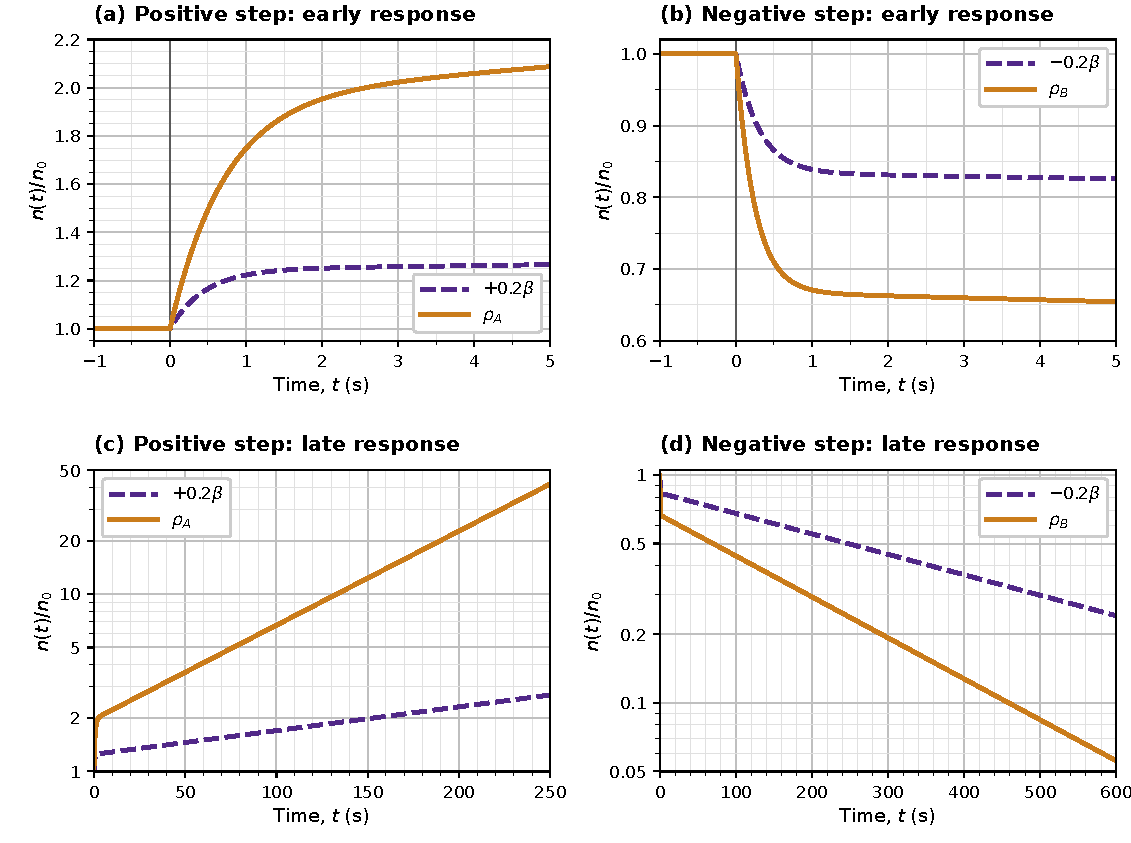
\includegraphics[width=\linewidth]{figures/lesson_27_traces.pdf}

\begin{enumerate}[itemsep=2pt,topsep=2pt]
\item From (a,b), estimate the apparent jump/drop factor $J$ for each curve.
      Use the settled trend after the fast adjustment; extrapolate gently
      toward $t=0$ if needed.
\item From the straight portions of (c,d), mark two widely separated points,
      estimate the \emph{signed} period $T$, and show your ruler construction.
\item Estimate $\rho_A/\beta$ and $\rho_B/\beta$ twice: from $J$ and from $T$.
      Check the known $\pm0.2\beta$ curves. Explain small disagreements.
\end{enumerate}

\begin{center}
\renewcommand{\arraystretch}{1.65}
\begin{tabularx}{.98\linewidth}{@{}lYYYY@{}}
\toprule
\textbf{Trace} & \textbf{$J$ from plot} & \textbf{$T$ (s) from plot} &
\textbf{$\rho/\beta$ from $J$} & \textbf{$\rho/\beta$ from $T$}\\
\midrule
$+0.2\beta$ & \RevealMath[.8in]{1.25} & \RevealMath[.9in]{+323} &
 \RevealMath[.8in]{+0.20} & \RevealMath[.8in]{+0.20}\\
$\rho_A$ & \RevealMath[.8in]{1.96\text{--}2.0} &
 \RevealMath[.9in]{+81.7} & \RevealMath[.8in]{+0.49\text{--}0.50} &
 \RevealMath[.8in]{+0.50}\\
$-0.2\beta$ & \RevealMath[.8in]{0.834} & \RevealMath[.9in]{-483} &
 \RevealMath[.8in]{-0.20} & \RevealMath[.8in]{-0.20}\\
$\rho_B$ & \RevealMath[.8in]{0.668} & \RevealMath[.9in]{-241} &
 \RevealMath[.8in]{-0.50} & \RevealMath[.8in]{-0.50}\\
\bottomrule
\end{tabularx}
\end{center}
\textbf{Discuss.} Why does the negative insertion not remove all neutrons
immediately? Which part of each response is governed by precursor decay?
Use $\rho_A$ and $\rho_B$ to practice conversion to dollars and pcm.
\end{document}
